\documentclass{article}

\usepackage{graphicx}
\usepackage{tikz}
\usepackage{tikzsymbols}
\usetikzlibrary{calc,patterns,shapes.geometric}
\pagestyle{empty}
\usepackage[margin=0pt]{geometry}
\geometry{papersize={14in,12in}}

\def\centerarc[#1](#2)(#3:#4:#5){\draw[#1] ($(#2)+({#5*cos(#3)},{#5*sin(#3)})$) arc (#3:#4:#5);}

\begin{document}
	\begin{figure}
		\centering
		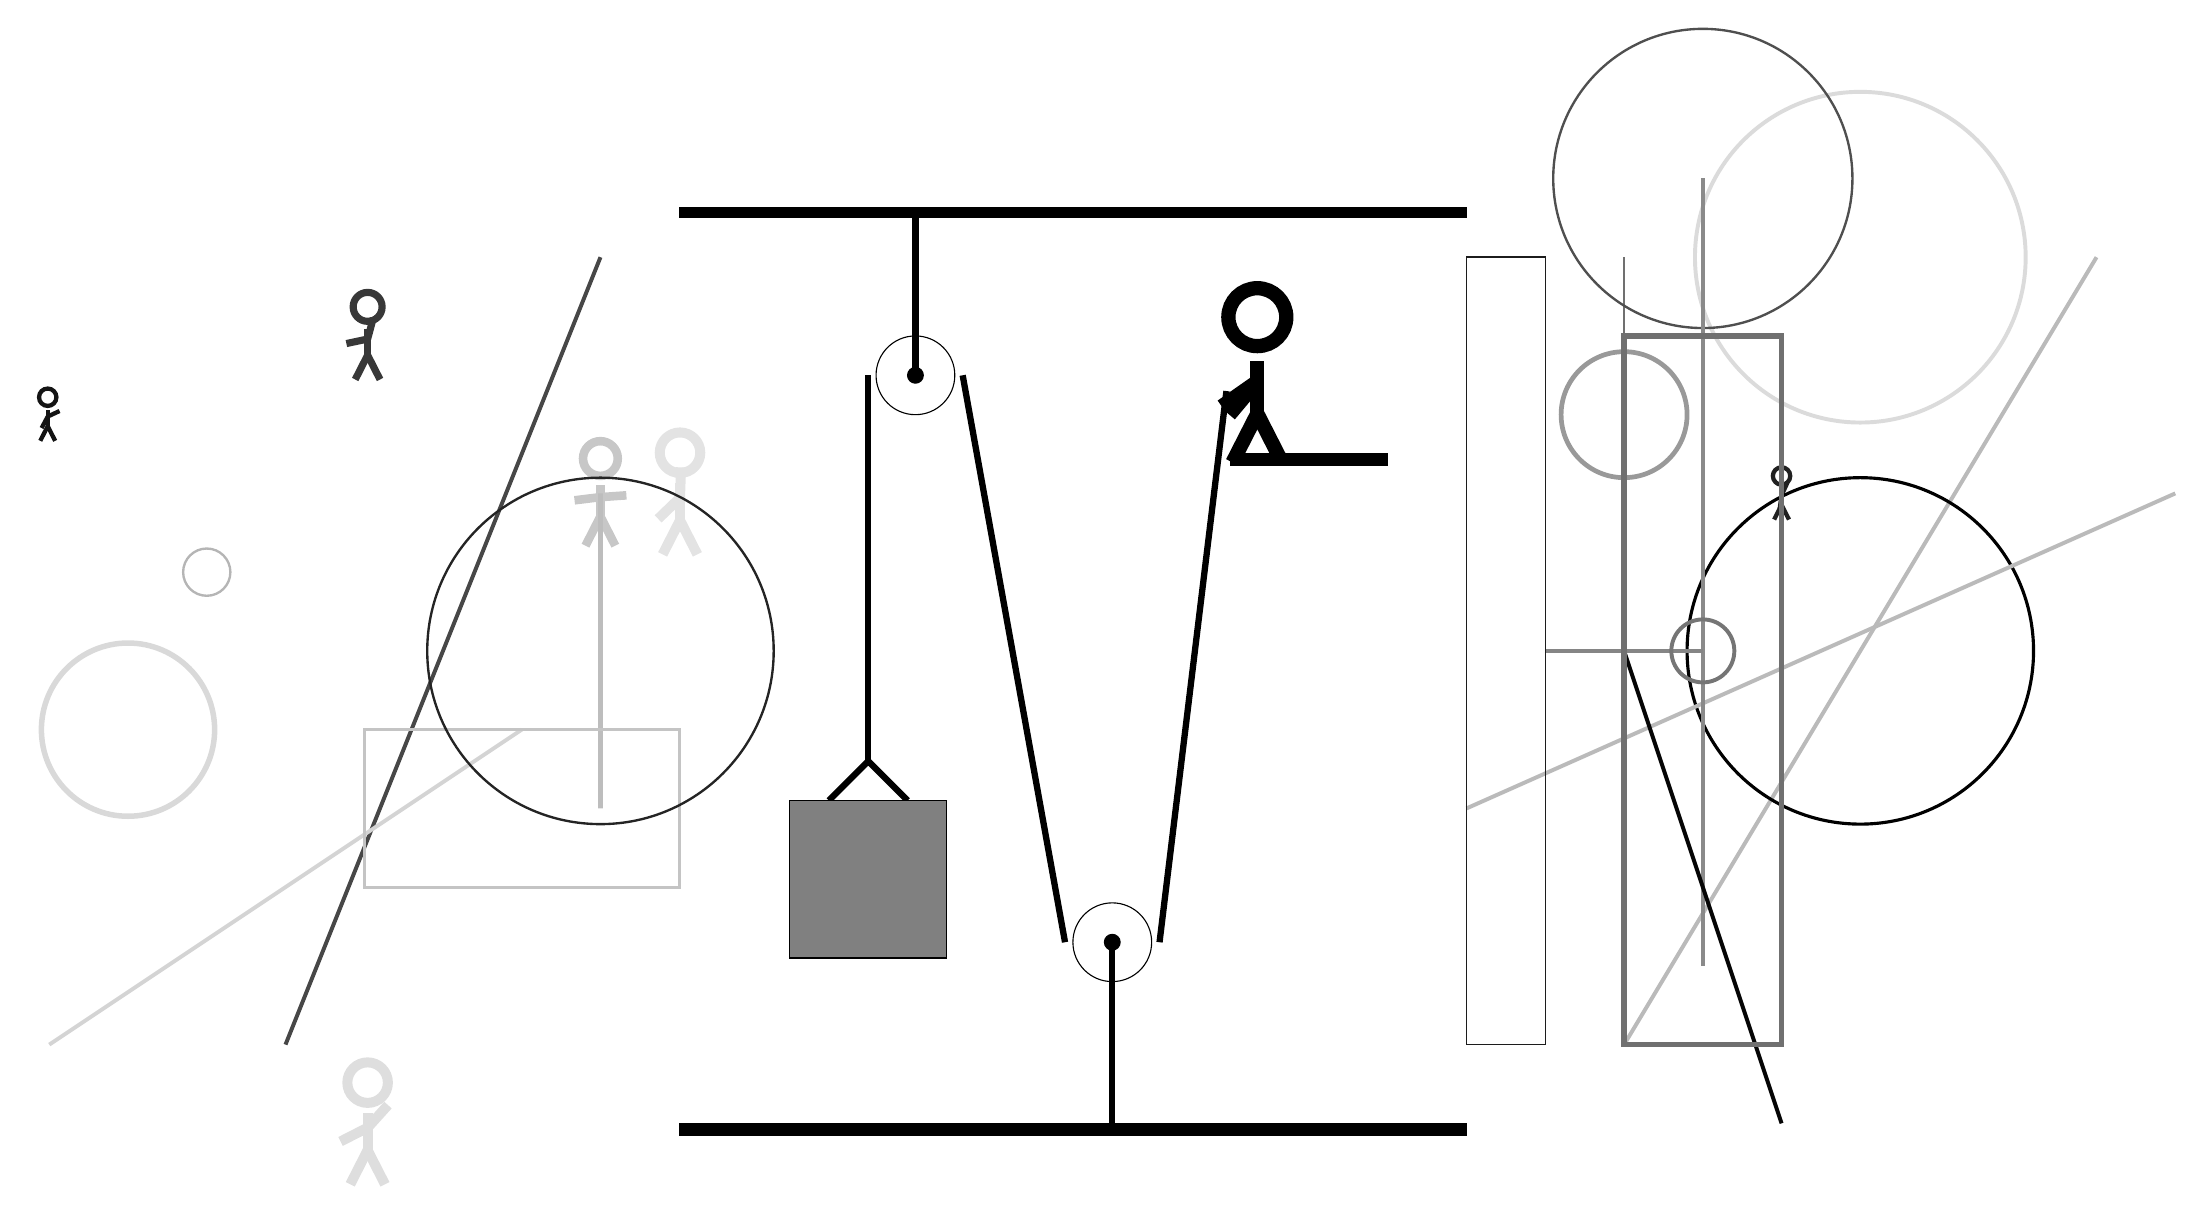
\begin{tikzpicture}
			%%%%% START %%%%%
			
			\draw[fill=black] (-2, 11.5) rectangle (8, 11.625);
			
			\draw (3.5, 2.3) circle (0.5);
			\draw[fill=black] (3.5, 2.3) circle (0.1);
			\draw[line width=0.8mm] (3.5, 2.3) -- (3.5, 0);
			
			\draw (1, 9.5) circle (0.5);
			\draw[fill=black] (1, 9.5) circle (0.1);
			\draw[line width=0.8mm] (1, 11.5) -- (1, 9.5);
			
			\draw[line width=0.3mm, color=black!56] (10, 11) rectangle (10, 1);
			
			\node[line width=0.3mm, color=black!87] at (12, 8) {\Strichmaxerl[3][82][65]};
			\node[line width=0.3mm, color=black!22] at (-3, 8) {\Strichmaxerl[6][7][4]};
			\draw [line width=0.5mm, color=black!14](13, 11) circle (2.1);
			\draw[line width=0.5mm, color=black!27](10, 1) -- (16, 11);
			\draw [line width=0.6mm, color=black!40](10, 9) circle (0.8);
			\draw [line width=0.3mm, color=black!69](11, 12) circle (1.9);
			\draw[line width=0.5mm, color=black!72](-7, 1) -- (-3, 11);
			\draw [line width=0.4mm, color=black!100](13, 6) circle (2.2);
			\node[line width=0.3mm, color=black!13] at (-6, 0) {\Strichmaxerl[7][27][48]};
			
			\draw[line width=0.5mm, color=black!27](8, 4) -- (17, 8);
			\node[line width=0.3mm, color=black!78] at (-6, 10) {\Strichmaxerl[5][12][75]};
			\draw[line width=0.5mm, color=black!46](11, 2) -- (11, 12);
			
			\draw[line width=0.5mm, color=black!17](-4, 5) -- (-10, 1);
			\draw[line width=0.5mm, color=black!48] (9, 6) rectangle (11, 6);
			\draw[line width=0.5mm, color=black!98](12, 0) -- (10, 6);
			
			\node[line width=0.7mm, color=black!11] at (-2, 8) {\Strichmaxerl[7][44][88]};
			\draw[line width=0.6mm, color=black!26] (-3, 4) rectangle (-3, 8);
			\draw[line width=0.2mm, color=black!89] (9, 11) rectangle (8, 1);
			\draw [line width=0.3mm, color=black!29](-8, 7) circle (0.3);
			\draw [line width=0.2mm, color=black!76](-2, 6) circle (0.0);
			
			\draw[line width=0.4mm, color=black!23] (-2, 3) rectangle (-6, 5);
			\draw[line width=0.5mm, color=black!82](12, 8) -- (12, 7);
			\draw[line width=0.7mm, color=black!56] (10, 1) rectangle (12, 10);
			\draw [line width=0.5mm, color=black!54](11, 6) circle (0.4);
			
			\node[line width=0.6mm, color=black!92] at (-10, 9) {\Strichmaxerl[3][62][25]};
			
			\draw [line width=0.3mm, color=black!86](-3, 6) circle (2.2);
			\draw [line width=0.7mm, color=black!15](-9, 5) circle (1.1);
			
			
			\draw[line width=0.8mm](-0.1, 4.1) --  (0.4, 4.6) -- (0.9, 4.1);
			\draw[fill=black!50] (-0.6, 4.1) rectangle (1.4, 2.1);
			
			\draw[line width=0.8mm](0.4, 9.5) -- (0.4, 4.6);
			\centerarc[line width=0.8mm](1, 9.5)(180:0:0.6)
			\draw[line width=0.8mm](1.6, 9.5) -- (2.9, 2.3);
			\centerarc[line width=0.8mm](3.5, 2.3)(180:360:0.6)
			\draw[line width=0.8mm](4.1, 2.3) -- (4.95, 9.3);
			
			\node at (5.3, 9.5) {\Strichmaxerl[10][35][-130]};
			\draw[fill=black] (5, 8.5) rectangle (7, 8.35);
			
			\draw[fill=black] (-2, 0) rectangle (8, -0.15);
			
			%%%%% END %%%%%
		\end{tikzpicture}
	\end{figure}	
\end{document}